\documentclass[a4paper, UKenglish, cleveref, autoref, thm-restate]{lipics-v2021}
\usepackage[utf8]{inputenc} % Required for inputting international characters
\usepackage[T1]{fontenc} % Output font encoding for international characters
% \usepackage[backend=bibtex,style=alphabetic,natbib=true]{biblatex}
% \usepackage[backend=bibtex,style=alphabetic,natbib=true]{biblatex}
% \addbibresource{references.bib}
\usepackage{amsmath, amssymb, amsfonts, amsthm, stmaryrd}
\usepackage{caption}
\usepackage{subcaption}
\usepackage{graphicx}
\usepackage{enumitem}
\usepackage{mathpartir}
\usepackage{bussproofs}
\usepackage{xparse}
\usepackage[usenames, dvipsnames]{xcolor}
\usepackage{lipsum}
\usepackage{xargs}
\usepackage{hyperref}
\usepackage{tikz-cd}
\usepackage{todonotes}
\usepackage{url}
\usepackage{xspace}
\usepackage{rotating}
\usepackage{quiver}
\usepackage{minted}
\usepackage{newunicodechar}

% \addbibresource{references.bib}
\usepackage{array}   % for \newcolumntype macro
\newcolumntype{C}{>{$}c<{$}} % math-mode version of "l" column type
\newcolumntype{L}{>{$}l<{$}} % math-mode version of "l" column type

% \usepackage{draftwatermark}
% \SetWatermarkText{Confidential}
% \SetWatermarkScale{4}
% \SetWatermarkColor[gray]{0.9}

\hypersetup{
  linktocpage,
  colorlinks,
  citecolor=BlueViolet,
  filecolor=red,
  linkcolor=Blue,
  urlcolor=BrickRed
}
\newcommand{\mpav}[1]{\textcolor{red}{\textsc{Marco}: #1}}
\newcommand{\dcas}[1]{\textcolor{red}{\textsc{David}: #1}}
\newcommand{\mvol}[1]{\textcolor{red}{\textsc{Michael}: #1}}
\newcommand{\proofcomment}[1]{\text{\{ #1 \}}}
\newenvironment{proofof}[1] {\begin{proof}[Proof of {#1}]}{\end{proof}}
\newcommand{\eqdef}{\stackrel{\mathrm{\Delta}}{=}}
\newcommand{\bnfeq}{\mathrel{::=}}
\newcommand{\defeq}{\triangleq}
\newcommand{\rul}[3]{\frac{#2}{#3}\;  {\textrulelabel{#1}}}
\newcommand{\den}[1]{\llbracket #1 \rrbracket}
\newcommand{\jud}[3]{#1 \vdash #2 : #3}
\newcommand{\bden}[1]{\llparenthesis#1 \rrparenthesis}
\newcommand{\bigslant}[2]{{\raisebox{.2em}{$#1$}\left/\raisebox{-.2em}{$#2$}\right.}}
\newcommand{\quotient}[2]{\bigslant{#1}{#2}}
\newcommand{\curry}{\Lambda}
\newcommand{\uncurry}{\begin{sideways}\begin{sideways}$\Lambda$\end{sideways}\end{sideways}}
\newcommand{\Bool}{\mathbb{B}}
\newcommand{\N}{\mathbb{N}}
\newcommand{\Nat}{\N}
\newcommand{\R}{\mathbb{R}}
\newcommand{\Sets}{\mathbf{Set}}
\newcommand{\blacklater}{\blacktriangleright}
\newcommand{\tot}{\mathcal{S}}
\newcommand{\PSh}{\ensuremath{\textbf{PSh}(\omega)}}

\newsavebox{\lbananabox}
\newcommand{\lbananamacro}{%
  
\begin{tikzpicture}[baseline=0.25em,xscale=0.005em,yscale=0.005em]
  \draw[solid, join=round] (2,0) to[out=140,in=-90] (0,3) to[out=90,in=-140] (2,6) -- (2.1,5.9)
              to[out=-120,in=90] (1.2,3) to[out=-90,in=120] (2.1,0.1) -- cycle;
\end{tikzpicture}
}
\savebox{\lbananabox}{\lbananamacro}
\newcommand{\lbanana}{\mathopen{\usebox{\lbananabox}\hspace{-0.6ex}}}


\newsavebox{\rbananabox}
\newcommand{\rbananamacro}{%
  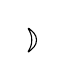
\begin{tikzpicture}[baseline=0.25em,xscale=-0.005em,yscale=0.005em]
  \draw[solid, join=round] (2,0) to[out=140,in=-90] (0,3) to[out=90,in=-140] (2,6) -- (2.1,5.9)
              to[out=-120,in=90] (1.2,3) to[out=-90,in=120] (2.1,0.1) -- cycle;
  \end{tikzpicture}
}
\savebox{\rbananabox}{\rbananamacro}
\newcommand{\rbanana}{\mathclose{\usebox{\rbananabox}}}


\newsavebox{\lbansbox}
\newcommand{\lbansmacro}{%
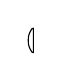
\begin{tikzpicture}[baseline=0.45ex,xscale=0.006em,yscale=0.012ex]%
% curvey bananas
%\draw[solid,join=round,fill=yellow] (2,0) to[out=140,in=-90] (0,3) to[out=90,in=-140] (2,6) -- (2.1,5.9) to[out=-120,in=90] (1.2,3) to[out=-90,in=120] (2.1,0.1) -- cycle;%
% fitted lenses
\draw[solid,join=round] (1.8,6) -- (1.5,5.9) to[out=-120, in=90] (0.7,3) to[out=-90, in=120] (1.5,0.1) -- (1.8,0) -- cycle;%
\end{tikzpicture}}
\savebox{\lbansbox}{\lbansmacro}
\newcommand{\lbans}{\mathopen{\usebox{\lbansbox}\mspace{1mu}}}

\newsavebox{\rbansbox}
\newcommand{\rbansmacro}{%
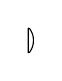
\begin{tikzpicture}[baseline=0.45ex,xscale=-0.006em,yscale=0.012ex]%
% curvey bananas
%\draw[solid,join=round,fill=yellow] (2,0) to[out=140,in=-90] (0,3) to[out=90,in=-140] (2,6) -- (2.1,5.9) to[out=-120,in=90] (1.2,3) to[out=-90,in=120] (2.1,0.1) -- cycle;%
% fitted lenses
\draw[solid,join=round] (1.8,6) -- (1.5,5.9) to[out=-120, in=90] (0.7,3) to[out=-90, in=120] (1.5,0.1) -- (1.8,0) -- cycle;%
\end{tikzpicture}}
\savebox{\rbansbox}{\rbansmacro}
\newcommand{\rbans}{\mathclose{\mspace{1mu}\usebox{\rbansbox}}}

\newsavebox{\llensbox}
\newcommand{\llensmacro}{%
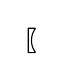
\begin{tikzpicture}[baseline=0.45ex,xscale=0.006em,yscale=0.012ex]%
\draw[solid,join=round] (1.4,0) -- (0,0) -- (0,6) -- (1.4,6) -- (1.5,5.9) to[out=-120, in=90] (0.7,3) to[out=-90, in=120] (1.5,0.1) -- cycle;%
\end{tikzpicture}}
\savebox{\llensbox}{\llensmacro}
\newcommand{\llens}{\mathopen{\usebox{\llensbox}\mspace{1mu}}}

\newsavebox{\rlensbox}
\newcommand{\rlensmacro}{%
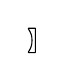
\begin{tikzpicture}[baseline=0.45ex,xscale=-0.006em,yscale=0.012ex]%
\draw[solid,join=round] (1.4,0) -- (0,0) -- (0,6) -- (1.4,6) -- (1.5,5.9) to[out=-120, in=90] (0.7,3) to[out=-90, in=120] (1.5,0.1) -- cycle;%
\end{tikzpicture}}
\savebox{\rlensbox}{\rlensmacro}
\newcommand{\rlens}{\mathclose{\mspace{1mu}\usebox{\rlensbox}}}

% filled versions
\newcommand{\Lbanana}{%
  \mathopen{\mspace{1mu}\tikz[baseline=0.25em,xscale=0.006em,yscale=0.006em]
  \fill (2,0) to[out=140,in=-90] (0,3) to[out=90,in=-140] (2,6) -- (2.1,5.9)
              to[out=-120,in=90] (1.2,3) to[out=-90,in=120] (2.1,0.1) -- cycle;\mspace{1mu}}}
\newcommand{\Rbanana}{%
  \mathclose{\mspace{1mu}\tikz[baseline=0.25em,xscale=-0.006em,yscale=0.006em]
  \fill (2,0) to[out=140,in=-90] (0,3) to[out=90,in=-140] (2,6) -- (2.1,5.9)
              to[out=-120,in=90] (1.2,3) to[out=-90,in=120] (2.1,0.1) -- cycle;}}
% % lens brackets (using TikZ)
% \newcommand{\llens}{%
%   \mathopen{\tikz[baseline=0.25em,xscale=0.006em,yscale=0.006em]
%   \draw[join=round] (1.4,0) -- (0,0) -- (0,6) -- (1.4,6) -- (1.5,5.9)
%         to[out=-120,in=90] (0.7,3) to[out=-90,in=120] (1.5,0.1) -- cycle;\mspace{1mu}}}
% \newcommand{\rlens}{%
%   \mathclose{\mspace{1mu}\tikz[baseline=0.25em,xscale=-0.006em,yscale=0.006em]
%   \draw[join=round] (1.4,0) -- (0,0) -- (0,6) -- (1.4,6) -- (1.5,5.9)
%         to[out=-120,in=90] (0.7,3) to[out=-90,in=120] (1.5,0.1) -- cycle;}}
% filled versions
\newcommand{\Llens}{%
  \mathopen{\tikz[baseline=0.25em,xscale=0.006em,yscale=0.006em]
  \fill (1.4,0) -- (0,0) -- (0,6) -- (1.4,6) -- (1.5,5.9)
        to[out=-120,in=90] (0.7,3) to[out=-90,in=120] (1.5,0.1) -- cycle;\mspace{1mu}}}
\newcommand{\Rlens}{%
  \mathclose{\mspace{1mu}\tikz[baseline=0.25em,xscale=-0.006em,yscale=0.006em]
  \fill (1.4,0) -- (0,0) -- (0,6) -- (1.4,6) -- (1.5,5.9)
        to[out=-120,in=90] (0.7,3) to[out=-90,in=120] (1.5,0.1) -- cycle;}}


\newcommand{\anamor}[1]{{\llens\, #1\, \rlens}}
\newcommand{\catamor}[1]{\lbans\, #1\, \rbans}
\newcommand{\cata}[1]{\lbans #1 \rbans}
\newcommand{\ana}[1]{\llens #1 \rlens}
\newcommand{\catafree}[1]{\Lbanana #1 \Rbanana}
\newcommand{\anacofree}[1]{\Llens #1 \Rlens}
\newcommand{\hylo}[2]{\cata{#1 \to #2}}
\newcommand{\cohylo}[2]{\ana{#1 \to #2}}
\newcommand{\fold}[1]{\catamor{#1}}
\newcommand{\unfold}[1]{\anamor{#1}}
\newcommand{\comp}{\cdot}
\newcommand{\operator}[1]{\textsf{#1}}
\newcommand{\head}{\operator{head}}
\newcommand{\inl}{\operator{inl}}
\newcommand{\inr}{\operator{inr}}
\newcommand{\tail}{\operator{tail}}
\newcommand{\Alg}{\text{-Alg}}
\newcommand{\Free}{\text{Free\xspace}}
\newcommand{\fmap}[1]{\text{fmap}\;#1}

\newcommand{\zero}{\operator{zero}}
\newcommand{\Nil}{\operator{nil}}
\newcommand{\Succ}{\operator{succ}}

\newcommand{\InOp}{\operator{in}^{\circ}}
\newcommand{\InIso}{\operator{in}}
\newcommand{\OutOp}{\operator{out}^{\circ}}
\newcommand{\OutIso}{\operator{out}}
\newcommand{\call}{\operator{call}}

\newcommand{\CatC}{\mathcal{C}}
\newcommand{\CatD}{\mathcal{D}}
\newcommand{\CatE}{\mathcal{E}}
\newcommand{\CatI}{\mathcal{I}}
\newcommand{\Set}{\mathbf{Set}}
\newcommand{\iso}{\cong}
\newcommand{\ceiling}[1]{\lceil #1 \rceil}
\newcommand{\floor}[1]{\lfloor #1 \rfloor}
\newcommand{\pair}[2]{\langle #1, #2 \rangle}
\newcommand{\haskell}[1]{\mintinline{haskell}{#1}}

\title{A Mechanised Library for Generic (Co)Programming}

\bibliographystyle{plainurl}% the mandatory bibstyle
%\titlerunning{Dummy short title} %TODO optional, please use if title is longer than one line

\author{Jane {Open Access}}{Dummy University Computing Laboratory, [optional: Address], Country \and My second affiliation, Country \and \url{http://www.myhomepage.edu} }{johnqpublic@dummyuni.org}{https://orcid.org/0000-0002-1825-0097}{(Optional) author-specific funding acknowledgements}%TODO mandatory, please use full name; only 1 author per \author macro; first two parameters are mandatory, other parameters can be empty. Please provide at least the name of the affiliation and the country. The full address is optional. Use additional curly braces to indicate the correct name splitting when the last name consists of multiple name parts.

\author{Joan R. Public\footnote{Optional footnote, e.g. to mark corresponding author}}{Department of Informatics, Dummy College, [optional: Address], Country}{joanrpublic@dummycollege.org}{[orcid]}{[funding]}

\authorrunning{J. Open Access and J.\,R. Public} %TODO mandatory. First: Use abbreviated first/middle names. Second (only in severe cases): Use first author plus 'et al.'

\Copyright{Jane Open Access and Joan R. Public} %TODO mandatory, please use full first names. LIPIcs license is "CC-BY";  http://creativecommons.org/licenses/by/3.0/

\ccsdesc[100]{\textcolor{red}{Replace ccsdesc macro with valid one}} %TODO mandatory: Please choose ACM 2012 classifications from https://dl.acm.org/ccs/ccs_flat.cfm 

\keywords{Dummy keyword} %TODO mandatory; please add comma-separated list of keywords

\category{} %optional, e.g. invited paper

\relatedversion{} %optional, e.g. full version hosted on arXiv, HAL, or other respository/website
%\relatedversiondetails[linktext={opt. text shown instead of the URL}, cite=DBLP:books/mk/GrayR93]{Classification (e.g. Full Version, Extended Version, Previous Version}{URL to related version} %linktext and cite are optional

%\supplement{}%optional, e.g. related research data, source code, ... hosted on a repository like zenodo, figshare, GitHub, ...
%\supplementdetails[linktext={opt. text shown instead of the URL}, cite=DBLP:books/mk/GrayR93, subcategory={Description, Subcategory}, swhid={Software Heritage Identifier}]{General Classification (e.g. Software, Dataset, Model, ...)}{URL to related version} %linktext, cite, and subcategory are optional

%\funding{(Optional) general funding statement \dots}%optional, to capture a funding statement, which applies to all authors. Please enter author specific funding statements as fifth argument of the \author macro.

\acknowledgements{I want to thank \dots}%optional

%\nolinenumbers %uncomment to disable line numbering



%Editor-only macros:: begin (do not touch as author)%%%%%%%%%%%%%%%%%%%%%%%%%%%%%%%%%%
\EventEditors{John Q. Open and Joan R. Access}
\EventNoEds{2}
\EventLongTitle{42nd Conference on Very Important Topics (CVIT 2016)}
\EventShortTitle{CVIT 2016}
\EventAcronym{CVIT}
\EventYear{2016}
\EventDate{December 24--27, 2016}
\EventLocation{Little Whinging, United Kingdom}
\EventLogo{}
\SeriesVolume{42}
\ArticleNo{23}
%%%%%%%%%%%%%%%%%%%%%%%%%%%%%%%%%%%%%%%%%%%%%%%%%%%%%%

\begin{document}

\maketitle

%TODO mandatory: add short abstract of the document
\begin{abstract}

\end{abstract}

\section{Introduction}
Recursive definitions cannot be proven well-defined automatically due to the
halting problem. Modern proof assistants like Coq or Agda provide a sound, but
incomplete algorithm which syntactically checks for termination or productivity.
For recursion, this is done by trying to (automatically) infer which argument in
the recursive call gets smaller with respects to the original input argument.
For productivity, the algorithm checks that the (co)recursive call appears
directly under a constructor to make sure that this function always produce at
least one element after each recursive step.

As mentioned, some functions, though well-defined, cannot be accepted by the
proof assistant. One example is the quicksort algorithm. This is given by the
\haskell{partition} and \haskell{quicksort} function below (written in Haskell
code):
\begin{minted}{haskell}
partition :: [a] -> ([a], a, [a])
partition (x:xs) = (filter (x <=) xs, x, filter (x >) xs)

quicksort :: [a] -> [a]
quicksort [] = []
quicksort ls = let (xs, x, ys) = partition ls in
                        (quicksort xs) ++ [x] ++ (quicksort ys)
\end{minted}
While \haskell{quicksort} is a well-defined mathematical function it cannot be
accepted by a proof assistant.  The reason is that the \haskell{partition}
function \emph{destructuring} the input ``dives'' deeper in the input returning
two sublists with the head as a pivot.

A pen-and-paper technique would be to show that the \haskell{partition} is a
\emph{well-founded coalgebra} on the functor $(- \times A \times -)$ for a fixed
type $A$. Here the term ``well-founded'' refers to the fact that the infinite
iteration of this coalgebra will produce a \emph{finite} binary tree with nodes
in $A$.

More generally, this is an instance of a \emph{divide-and-conquer} algorithm.
Such algorithms are structured in three parts: first, the input is broken down
in smaller sub-problems by means of a well-founded coalgebra. Secondly, these
sub-problems are computed recursively and, finally, the results of the recursive
call are put together by a an algebra. This particular way of doing recursion
has been named in the functional programming literature as a
hylomorphism~\cite{MeijerFP91, HuIT96}.

Many years later Hinze et al.~\cite{HinzeWG15} showed that every recursive
program can be turned into an hylomorphism by means of the conjugate rule. The
essence of this result is that every complex recursion scheme can be explained
by its associated \emph{adjunction} which establishes a way of reducing the
proof obligation for the complex recursion scheme into the proof obligation for
a basic hylomorphism. This can be paraphrased by saying
\begin{center}
  ``\emph{every recursion scheme can be formalised as an hylomorphism}''
\end{center}

This result has given a much needed unifying view of recursion scheme which
helped understanding their nature and also in providing a unified way of
reasoning about recursive programs by means of fusion laws.

\dcas{My take would be different here from now on. See below:}

Recursion schemes enjoy generic algebraic laws for program manipulation. Many
common optimisations and transformations are instances of such laws. Examples of
this include shortcut deforestation~\cite{TakanoM95}, and
parallelisations~\cite{Gibbons96:Third}. \dcas{TODO: add more examples?}

With this work, we study the formalisation of hylomorphism laws in proof
assistants like Coq to derive efficient and correct recursive algorithms by
program calculation techniques. Furthermore, our encoding of hylomorphisms
allows Coq's code extraction mechanism to produce OCaml code that resembles what
a programmer would have writen manually.

\dcas{END (TODO: merge with Marco's. I would omit (or take parts of the) below)}

There is a tension:
\begin{itemize}
  \item On one hand we can allow general recursion and the employ recursion
schemes to help the programmer structuring programs so that they terminate
  \item on the other hand we could forbid non-termination, but at this point
there is no algorithm to tell termination and non-termination apart.
\end{itemize}

The type theoretical approach instead is to reject all definitions which cannot
be proven well-defined. It is safer, but incomplete.

With this work we intend to begin a study of the applications of recursion
schemes that goes beyond functional programming, that is to dependent type
theories such as a the ones employed in proof assistants like Agda or Coq where
non-termination is outright rejected.

This has been a long-standing challenge to come up with a sound algorithm which
rejects all programs that do not terminate (soundness) and accepts as many
well-defined programs as possible (completeness). Our aim is to provide an
additional tool to the every-day programmer to be able to extend the range of
recursive programs we can write.

\dcas{Note: the below is useful to keep in the intro}
One of the challenges here is to be able to keep the theory of recursions
schemes as general as possible while maintaining its practical usefulness. In
order to do this, we have to make some design choices which differ a bit from
the general theory.  For instance, formalising the conjugate rule would require
us to mechanise a non-trivial fragment of category theory inside the prover's
logic.  Secondly, the general conjugate rule is a statement of correspondence of
arrows rather than a proof that these programs actually exists. In functional
programming languages like for instance Haskell this is not a problem, since
every functor is strong and has a fixed-point.  On the other hand, in a type
theory we have to restrict to those so-called polynomial functors. In this work
we do not make use of these assumptions. By restricting ourselves to polynomial
functors given in terms of containers~\cite{AbbottAG05} we are able to prove the
recursion schemes within the proof assistant and at the same time to maintain a
certain level of data abstraction.

First we prove that the hylo equation has a unique solution
\[
  x = a \comp F(x) \comp c
\]
for every recursive coalgebra $c$ for a polynomial $F$. Then we prove each
recursion scheme by reducing it to a hylo. The following recursion schemes can
all be proven by reducing them to an hylo: folds, mutual recursive functions,
recursion schemes from comonads and their respective coinductive dual.

The contributions we make in this paper are as follows:
\begin{itemize}
  \item We provide a framework for \emph{generic programming} with recursion
schemes in Coq
  \item We formalise algorithms for divide and conquer, dynamic programming and
mutual recursion
  \item We validated optimisations in Coq and extract the resulting code to
OCaml.
\end{itemize}

\section{Recursive Equations}

\subsection{Catamorphisms and Anamorphism}
A catamorphism is the unique program defined as
\[
  x = a \comp \fmap{x} \comp \InOp
\]
Can be implemented:
\[
  \cata{a} = \hylo{\InOp}{a}
\]

An anamorphism is the unique program satisfying the equation
\[
  x = \OutOp \comp \fmap{x} \comp{c}
\]
The anamorphism is indicated by $\ana{c}$. Recursion schemes given by a
corecursive algebra such as $\OutIso$ are also called hylomorphism but they are
indicated with the symbol for the anamorphism, $\cohylo{c}{\OutOp}$.

\paragraph{Free Monads}
Given an endofunctor $D$ and a type $A$ the free monad is defined as the least
solution to the following domain equation
\[
  D^{*}A = A + DD^{*}A
\]
where $\eta_{A} : A \to D^{*}A$ is the left injection and
$\call_{A} : DD^{*}A \to D^{*}A$ is the right injection. Given an algebra
$a : DA \to A$ there is a unique solution to the following recursive equation
\[
  x \comp \call_{A} = a \comp D(x)
\]
that is $\catafree{a} = \cata{[id_{A}; a]}$. With this operation we can extend
the free algebra $\call$ to the multiplication $\mu : D^{*}D^{*}A \to D^{*}A$
defined as $\mu = \catafree{\call}$.

\paragraph{Cofree Comonads}
Given an endofunctor $D$ and a type $A$ the cofree comonad is defined as the
greatest solution to the following domain equation
\[
  D_{\infty}A = A + DD_{\infty}A
\]
where $\head : D_{\infty}A \to A$ is the first projection and
$\tail_{A} : D_{\infty}A \to DD_{\infty}A$ is the second projection.
Given an algebra $c : A \to DA$ there is a unique solution to the following
recursive equation
\[
  \tail_{A} \comp x = D(x) \comp c
\]
that is $\anacofree{c} = \ana{\pair{id_{A}}{c}}$. With the latter operation we
can extend $\tail$ to the comultiplication for the comonad
$\delta : D_{\infty}A \to D_{\infty} D_{\infty}A$ defined by
$\delta = \anacofree{\tail}$.


\subsection{Accumulators}
For an algebra $a : D(A^{P})\times P \to A$:
\begin{align*}
  & g : \mu D \times P \to B\\
  & g (d, p) = a (\fmap{(\curry g)} \comp \InOp(d), p)
\end{align*}

\paragraph{Hylo Implementation}
Given an algebra $a : D(A^{P}) \to A^{P}$ the accumorphism corresponds to the unique
solution to the following equation
\begin{align*}
  & f : \mu D \to A^{P}\\
  & f = a \comp \fmap (f) \comp \InOp
\end{align*}
thus $f = \hylo{\InOp}{a}$.

The complex recursion scheme is then
$g = \uncurry\hylo{\InOp}{a} : \mu D \times P \to B$.

\subsection{Mutu-Hylo}
For an algebra $a_{1} : D(A_{1} \times A_{2}) \to A_{1}$ and an algebra
$a_{2} : D(A_{1} \times A_{2}) \to A_{2}$:
\begin{align*}
  & (g_{1}, g_{2}) : (\mu D, \mu D) \to (A_{1}, A_{2})\\
  & (g_{1}, g_{2}) = (a_{1}, a_{2}) \comp (\fmap{\pair{g_{1}}{g_{2}}},\fmap{\pair{g_{1}}{g_{2}}}) \comp (\InOp, \InOp)
\end{align*}

\paragraph{Hylo Implementation}
Given an algebra $a : D(A_{1} \times A_{2}) \to A_{1} \times A_{2}$
\begin{align*}
  & f : \mu D \to A_{1} \times A_{2}\\
  & f = a \comp \fmap{f} \comp \InOp
\end{align*}
for which the solution is an hylo $f = \hylo{\InOp}{a}$.

The mutumorphism can be implemented as
$(g_{1}, g_{2}) = (\pi_{1} \comp f, \pi_{2} \comp f)$.

\paragraph{Coq Implementation}
Given the two algebras  $a_{1} : D(A_{1} \times A_{2}) \to A_{1}$ and
$a_{2} : D(A_{1} \times A_{2}) \to A_{2}$.
We define the two recursive functions  $f_{1}$ and $f_{2}$ as

\[
  f_{1} = \pi_{1} \comp \hylo{\InIso}{\pair{a_{1}}{a_{2}}} \qquad f_{2} = \pi_{2} \comp \hylo{\InIso}{\pair{a_{1}}{a_{2}}}
\]

\subsubsection{Example}
Say that we want to prove that the two functions below are well-defined

\begin{tabular}{LL}
  \operator{even} : \Nat \to \Bool                  &  \operator{odd} : \Nat \to \Bool\\
  \operator{even} (0) = \top                        &  \operator{odd}(0) = \bot\\
  \operator{even} (n+1) = \neg \operator{odd}(n)    &  \operator{odd}(n+1) = \neg (\operator{even}(n))
\end{tabular}

One option is to prove that the following function (given by a catamorphism) is
equivalent to the above
\begin{align*}
  & \operator{even-odd} : \Nat \to \Bool \times \Bool\\
  & \operator{even-odd} (0) = (\top, \bot)\\
  & \operator{even-odd} (n+1) = \operator{let } (x,y) \leftarrow \operator{even-odd}(n) \operator{ in } (\neg x, \neg y)
\end{align*}
This function is clearly a catarmorphism:
\begin{align*}
  & \operator{even-odd} : \Nat \to \Bool \times \Bool\\
  & \operator{even-odd} = \cata{a} \operator{ where }\\
  & \qquad \qquad a : 1 + (\Bool \times \Bool)\\
  & \qquad \qquad a (\Nil) = (\top, \bot)\\
  & \qquad \qquad a (\operator{x,y}) = (\neg x, \neg y)
\end{align*}
where $\cata{\cdot}$ takes a $(1+-)$ algebra on $\Bool \times \Bool$ and returns
the associated recursive function.

Now we recover the original two functions by setting
$\operator{even}' \eqdef \pi_{1} \comp \operator{even-odd}$
$\operator{odd}' \eqdef \pi_{2} \comp \operator{even-odd}$. The proof that these
two pairs of functions are the same is an easy induction over the natural
numbers.

This is an instance of a more general phenonema whose argumet uses category
theory.

\subsection{Course-of-Value Recursion}
The knapsack algorithm is defined as following in pseudo-Haskell code:
\begin{align*}
  & \operator{knapsack} : [(\Nat, \R)] \to \Nat \to \R\\
  & \operator{knapsack}\;wvs\; c = \operator{maximum}_{0}
    [v + \operator{knapsack}\;wvs\; (c - w) \mid (w,v) \leftarrow wvs, w \le c]
\end{align*}
%
with dynamic programming knapsack can be rephrased like this
\begin{align*}
  & \operator{knapsack} : [(\Nat, \R)] \to \Nat \to \R\\
  & \operator{knapsack}\;wvs\;c= table !! c \\
  & \qquad table  = [ks\;i \mid i \leftarrow [0..c]]\\
  & \qquad ks\; i = maximum_{0} [v + table!! (i - w) \mid (w,v) \leftarrow wvs, w \le i]
\end{align*}

The recursion scheme is justified by solving a recursive equation.  First we
define an operation to create a memory table representing the list of capacities
$[0..c]$. We first define a functor $D X = 1 + X$ representing the base functor
for constructing the naturals $\Nat = \mu D$ the we define the generating
function by induction on the naturals
\begin{align*}
  & \operator{fan} : \Nat \to D_{\infty}\Nat\\
  & \operator{fan} (0)    = \pair{0}{\inl}\\
  & \operator{fan} (n+1)  = \pair{n+1}{\inr (\operator{fan}(n))}
\end{align*}
The recursion scheme from a comonad is then defined as follows
\begin{align*}
  & \operator{rsfc} : \Nat \to A\\
  & \operator{rsfc} = alg \comp DD_{\infty}(\operator{rsfc}) \comp D(\operator{fan}) \comp \InOp
\end{align*}
At his point we can given the definition of the algebra $alg$ which effectively implements knapsack.
Firs we define the $\operator{lookup}$ function which returns (if present) the element indexed in the memory table
\begin{align*}
  & \operator{lookup} : \Nat \to D_{\infty} \R \to \R_{\bot}\\
  & \operator{lookup} (0,   \pair{r}{\textunderscore})  = r\\
  & \operator{lookup} (n+1, \pair{r}{\inl})         = \bot\\
  & \operator{lookup} (n+1, \pair{r}{\inr(table)})  = \operator{lookup} (n, table)
\end{align*}
and now we can define the algebra over the reals
\begin{align*}
  & \operator{alg} : DD_{\infty} \R \to \R\\
  & \operator{alg}\; (\inl)  = 0\\
  & \operator{alg}\; (\inr(table))  = \operator{maximun}_{0} [ v + \operator{lookup}\; table\; (i - w) \mid (w,v) \leftarrow wvs, w \le i]
\end{align*}

It remains to show how an $\operator{rsfc}$ is implemented in terms of
hylomorhisms.

\paragraph{Implementation into hylomorphisms}
In order to implement rsfcs as hylos we need a parametric distributive law
\[
  \lambda_{X} : GG_{\infty}X \to G_{\infty}GX
\]
This can be defined as
$\lambda = G_{\infty}G(\head) \comp \anacofree{G(\tail)}$.  The distributive law
is instrumental to be able to lift coalgebras in the following sense. Give a
$G$-coalgebra on $X$, a lifting $H$ is a functor which lifts this coalgebra to a
$G$-coalgebra on $HX$.  In particular, the lifting $G_{\lambda}$ takes
$G_{\infty}$-coalgebras on $X$ and transforms them into $G_{\infty}$-coalgebras
on $GX$
\begin{align*}
  & G_{\lambda}(c) : GA \to G_{\infty} GA\\
  & G_{\lambda}(c) = \lambda \comp G (c)
\end{align*}
where $c : C \to GC$.

Now, given an algebra $a : GG_{\infty} A \to A$ on the carrier $A$ we can
convert it into an algebra for the carrier $G_{\infty} A$ by
\begin{align*}
  & \floor{a} : GG_{\infty} A \to G_{\infty} A\\
  & \floor{a} = G_{\infty}(a) \comp \anacofree{G_{\lambda}(\delta)}
\end{align*}
where $\eta_{A} : A \to G_{\infty} A$ is the unit of the comonad creating an
infinite constant list.

At this point the hylo is simply defined by
$\hylo{\InOp}{a} : \mu F \to G_{\infty}A$  and the rsfc is derived as follows
\begin{align*}
  & \operator{rsfc} : \mu G \to A \\
  & \operator{rsfc} = \head \comp \hylo{\InOp}{a}
\end{align*}

% A recursion scheme from a comonad $D_{\infty}$ for a data functor $F$

% For example, for the functor $(1 + -)$ an algebra over this functor is a
% function $1 + X \to X$ is a pair of functions $\Nil : 1 \to X$ and
% $\Succ : X \to X$. The cofree comonad over $D$ is defined as follows
% \[
%   D_{\infty} A \iso A \times (1 + D_{\infty})
% \]
% which is the the type of non-empty possibly infinite lists with elements in $A$


% First we have to assume a distributive law
% $\lambda : DD_{\infty} \to D_{\infty}D$.  For an algebra
% $a : D(D_{\infty} A) \to A$,
% \begin{align*}
%   & g : \mu D \to A\\
%   & g = a \comp D(G_{\infty}(g) \comp \anacofree{\cata{G^{\lambda}(\InIso)}}) \comp \InOp
% \end{align*}
% where
% $G^{\lambda} (alg : D\mu F \to \mu F) = DGX \xrightarrow{\lambda} GDX \xrightarrow{G(alg)} GX$
% is a $D$-algebra on $GX$. The catamorphism of this algebra has the following
% type
% \[
%   \cata{G^{\lambda}(\InIso)} : \mu D \to G\mu D
% \]
% which is the type of a $G$-algebra used to initialise the memory table.

% Given an algebra $a : DG_{\infty} A \to G_{\infty} A$ we can equivalently ask
% what is the unique solution of the following equation
% \begin{align*}
%   & f : \mu F \to G_{\infty} A\\
%   & f = a \comp \fmap{f} \comp \InOp
% \end{align*}
% The solution to this equation can be found again using an hylo
% $f = \hylo{\InOp}{a} : \mu F \to G_{\infty} A$.  The course-of-value recursion
% can be recovered from this by setting $g = \head \comp f$

% \subsubsection{Histomorphism}

% The definition of $\lambda$ is:
% \begin{align*}
%   & \lambda : GG_{\infty} A \to G_{\infty} GA\\
%   & \lambda = \fmap{(\fmap{\head})}\comp \anacofree{\fmap{\tail}}
% \end{align*}
% For example, for $GX = 1 + X$ we have to define
% \begin{align*}
%   & \lambda : 1 + G_{\infty} A \to G_{\infty} (1 + A)\\
%   & \lambda(\inl) = \pair{\inl}{\lambda(\inl)}\\
%   & \lambda(\inr(table)) = \pair{\inr (\head(table))}{\lambda (\tail (table))}
% \end{align*}


% % \begin{align*}
% %   & \operator{lookup} :: \Nat \to G_{\infty} \R \to \operator{Maybe}\;\R\\
% %   & \operator{lookup}\; \Zero       (\Cons{a}{\text{\textunderscore}})     = \Just{a}\\
% %   & \operator{lookup}\; (\Succ{n})  (\Cons{a}{\Zero})                      = \Nothing\\
% %   & \operator{lookup}\; (\Succ{n})  (\Cons{a}{\Succ table})                = \operator{lookup}\; n  table
% % \end{align*}

% % Defining the algebra
% % \begin{align*}
% %   & \operator{alg} :: D (G_{\infty} \R) \to \R\\
% %   & \operator{alg}\; Zero           = 0\\
% %   & \operator{alg}\; (Succ{table}) = maximum_{0} [v + \operator{lookup}\; table (i - w) | (w,v) \leftarrow wvs, w \le i]
% % \end{align*}

\subsection{Course-of-Value Recursion with Finite Memory Table}
It can be proven that if $c$ is a recursive coalgebra, then the hylomorphism for
any algebra $a$ generates a finite output.  In other words, as far as the
hylomorphism is concerned $G_{\infty}$ can be regarded as its finite version
\[
  G_{*} A = \mu X. A \times G X
\]
We now rewrite course-of-value recursion using the finite memory table
For an algebra $a : D(D_{*} A) \to A$,
\begin{align*}
  & g : \mu F \to A
  & g = a \comp D(G_{*}(g) \comp \anacofree{\cata{G^{\lambda}(\InIso)}}) \comp \InOp
\end{align*}


\section{Mechanising Extractable Container Functors}

\dcas{Subsections are tentative topics to remember what I need to fill in here,
but these are not final}

Our mechanisation works in the category of Coq types, and our goals are: (1)
the mechanisation of hylomorphisms and their laws should be axiom-free; and (2)
Coq hylomorphisms should be extracted to recursive OCaml functions that use no
instances of \mintinline{OCaml}{Obj.magic}.  Although the use of
\mintinline{OCaml}{Obj.magic} is safe in the code extracted by Coq, it has been
proven that, for higher-order programs, simple interoperations can lead to
incorrect behaviour or even segfaults~\cite{forster:hal-04329663}.  Therefore,
the avoidance of axioms and  \mintinline{OCaml}{Obj.magic} means that the
extracted code will have stronger safety guarantees, and will allow the safe
interoperation with other OCaml code.

\subsection{Functors and Containers}

In Coq, to construct least/greatest fixpoints of functors, these need to build
\emph{strictly positive types}. A common approach to construct such strictly
positive endofunctors is to use \emph{container functors}~\cite{Whatever}.
However, reasoning about container and container functor equality requires to
consider: (a) functional extensionality; (b) heterogeneous equality. This is
problematic, due to our goals to remain axiom-free. Furthermore, standard
representations of containers in Coq will lead to OCaml code that contains
\mintinline{OCaml}{Obj.magic}. We will explain why, and our mechanisation of
containers in the remainder of this section.

A container is defined by a type of \emph{shapes}, and a \emph{family of
position types} indexed by shapes. 
\begin{minted}{Coq}
Context (Shape : Set) (Pos : Shape -> Set).
\end{minted}
An \emph{extension} of this container is a functor,
whose action on objects is given by:
\begin{minted}{Coq}
Record App (X : Set) := { shape : Shape; contents : Pos shape -> X }.
\end{minted}
In our mechanisation, we use \mintinline{Coq}{App} to represent container
extensions.  Generally, any functor that is isomorphic to a container extension
is called a \emph{container functor}. However, in our work we will call
\emph{container functor} to the functors defined by a specific container
extension.

The first problem in extracting Coq code from such container extensions is the
use of families of types. Since OCaml's type system cannot accurately capture
such families of types, Coq's code extraction mechanism will insert unsafe
casts. To avoid unsafe casts, we can consider representing the positions of a
container as a type that captures \emph{all} the potential positions in all
possible shapes, together with a predicate \mintinline{Coq}{Valid} that
determines whether a position is valid in a shape. 
\begin{minted}{Coq}
Context (Shape : Set) (Pos : Set) (Valid : Shape -> Pos -> Prop).
Record App (X : Set) := { shape    : Shape; 
                          contents : {p | Valid shape p} -> X }.
\end{minted}
This approach solves the the problem of the unsafe casts, since the code
extracted for \mintinline{Coq}{{p | Valid shape pos}} will be an OCaml
singleton type defined as the OCaml equivalent to \mintinline{Coq}{Pos}.

However, there still remains the issue of reasoning about the equality of
container extensions. The contents of the container extensions need to be
accessed via a function \mintinline{Coq}{contents}. The domain of this function
depends on the shape of the container. This means that, for a given type of
shapes and positions, the equality of two objects of a container extension will
need to deal with heterogeneous equality. Since we want to remain axiom-free,
one way to deal with this is to rely on a \emph{decidable} validity predicate.
This way, we reach our final definition for container extensions. First,
containers are defined as pairs of shape and position types that have a
\emph{decidable} validity predicate. We represent decidable predicates as
functions that return a boolean, and lift booleans to propositions similarly to
SSReflect. For simplicity, we define the dependent pair of valid positions as a
record, which will be extracted to a singleton type with the validity proof
erased by Coq's code extraction mechanism.
\begin{minted}{Coq}
Class Cont (Shape : Set) (Pos : Set) := { valid : Shape -> Pos -> bool }.
Coercion is_true (b : bool) : Prop := b = true.
Record PosOf `(C : Cont Shape Pos) (shape : Shape) := 
  ValidPos { val : Pos; IsValid : valid shape pos }.
\end{minted}
Then, we define \emph{container extensions} as
\begin{minted}{Coq}
Record App `(C : Cont Shape Pos) (X : Set) :=
  { shape : Shape; contents : PosOf C shape -> X }.
\end{minted}
The functorial action for container extensions on morphisms boils down to
function composition, which trivially preserves identity and composition.
\begin{minted}{Coq}
Definition fmap `(C : Cont Shape Pos) `(f : A -> B) (x : App C A) : App C B
  := {| shape := shape x; contents := fun e => f (contents x e) |}
\end{minted}

\subsubsection{Polynomial Functors as Container Extensions}

Polynomial functors can be defined as container extensions~\ref{fig:poly}. We
omit here the proofs that these container extensions are isomorphic to
polynomials, but this proof is straightforward. To illustrate how the identity,
constant, sum and product container extensions work, consider the
tree-generating functor (i.e.\ the functor whose fixpoint is a binary tree):
$F\; X = \mathbb{N} + X \times X$.

This functor is built as the sum of two functors: $X \mapsto \mathbb{N}$ and $X \mapsto
X \times X$. Consider first $X \mapsto \mathbb{N}$. This is a constant functor
that maps $X$ to the type $\mathbb{N}$. More generally, a functor that, given a
type $A$, maps everything to it, $X \mapsto A$, only needs one shape ($A$, L9
of Fig~\ref{fig:poly}), and zero positions (In Coq, \mintinline{Coq}{False},
L10 of Fig~\ref{fig:poly}). The reason why there are zero valid positions in
a constant container extension is because, given something of type 
\mintinline{Coq}{App (Const (Ks A) Kp) X}, it should be impossible to get
something of type \mintinline{Coq}{X}. But from the container shape, we will
always be able to get the element of type $A$\footnote{%
  Our decision to use \mintinline{Coq}{False} is arbitrary. In general, we
  could have chosen any time, with a validity predicate that always returns
  \mintinline{Coq}{false}. It would make no difference for code extraction.
}. This functor is, therefore \mintinline{Coq}{Const nat}.

Consider now $X \mapsto X \times X$. This is the product of two
identity functors $X \mapsto X$. The identity functor only has one shape, and
we can use the unit type to represent such shapes. From this shape we should be
able to get an element of type $X$, and we can capture this by using the unit
type for positions. To build an element of the container extension type, we
will need to provide a function of type \mintinline{Coq}{unit -> X}, which is
isomorphic to \mintinline{Coq}{X}. 

The shape of the product of two container extensions is the product of their
shapes. The product of such container extensions should allow us to get either
the left, or the right element in the product. Therefore, the positions of this
container extension is the sum of the positions of the two container
extensions. What is a valid position in a given shape? If the position is
\mintinline{Coq}{inl p} (or \mintinline{Coq}{inr p}), then it is only valid if
\mintinline{Coq}{p} is valid in the first (resp. second) component of the
shape. The product of our two container extensions is
\mintinline{Coq}{Prod Id Id}. 

Finally, the shape the sum of two container extensions is the sum of their
shapes. The positions are, like for products, the sum of their shapes. But to
check the validity of shapes in positions, their constructor must match, e.g.
shape \mintinline{Coq}{inl s} and shape \mintinline{Coq}{inl p}, with
\mintinline{Coq}{valid s p}. 

Our final container extension is the following: 
\mintinline{Coq}{Sum (Const nat) (Prod Id Id)}.
The shape of this functor is: 
\mintinline{Coq}{nat + unit * unit}. The positions of this functor
are \mintinline[breaklines]{Coq}{False + (unit + unit)}, which is isomorphic
to \mintinline{Coq}{unit + unit}, which will only be valid in the RHS.

The Coq value \mintinline{Coq}{inl n} of type
\mintinline{Coq}{nat + bool * bool} would look as follows as a container
extension 
\mintinline{Coq}{App (Sum (Const nat) (Prod Id Id)) bool}:
\begin{minted}{Coq}
{| shape := inl n; cont := fun e => uninhabited e|}
\end{minted}
We omit the definition of \mintinline{Coq}{uninhabited}, which exploits the
fact that \mintinline{Coq}{e} for \mintinline{Coq}{inl n} implies
\mintinline{Coq}{False} to build an element of type \mintinline{Coq}{bool}%
\footnote{Note that, since \mintinline{Coq}{e} is uninhabited we could return
any arbitrary value instead of \mintinline{Coq}{uninhabited e}.}.

Similarly, the Coq value \mintinline{Coq}{inr (true, false)} as a container
extension is as follows:
\begin{minted}{Coq}
  {| shape := inr (tt,tt);
     cont := fun e : {p | valid (inr (tt, tt)) p} =>
        match proj1_sig e with
        | inl f => match f with end
        | inr (inl tt) => fun _ => true
        | inr (inr tt) => fun _ => false
        end
  |}
\end{minted}
Here, the position \mintinline{Coq}{inl f} is impossible, as
\mintinline{Coq}{f} would need to be a proof of \mintinline{Coq}{False}.
Of the two remaining positions, the left one will return 
\mintinline{Coq}{true}, and the right position \mintinline{Coq}{false}.
\begin{figure}
\begin{minipage}{.52\textwidth}
  \begin{minted}[linenos, fontsize=\small]{Coq}
Context `(C1 : Cont S1 P1) 
        `(C2 : Cont S2 P2).

Definition Is := unit.
Definition Ip := unit.
Instance Id : Cont Is Ip := {
  valid := fun _ _ => true }.

Definition Ks (A : Set) := A.
Definition Kp := False.
Instance Const A : Cont (Ks A) Kp := {
  valid := fun _ p =>
    match p with end }.

Definition Ps : Type := S1 * S2.
Definition Pp : Type := P1 + P2.
Instance Prod : Cont Ps Pp := {
  valid := fun s p => 
    match p with
    | inl p' => valid (fst s) p'
    | inr p' => valid (snd s) p'
    end }.
\end{minted}
\end{minipage}
\begin{minipage}{.47\textwidth}
  \begin{minted}[linenos, firstnumber=23, fontsize=\small]{Coq}
Definition Ss : Type := S1 + S2.
Definition Sp : Type := P1 + P2.
Instance Sum : Cont Ss Sp := {
  valid := fun s p => 
    match s, p with
    | inl s', inl p' => valid s' p'
    | inr s', inr p' => valid s' p'
    | _, _ => false
    end }.

Definition Cs : Type := App F S2.
Definition Cp : Type := P1 * P2.
Instance Comp : Cont Cs Cp := 
{ valid :=  
    fun (s : App F S2) (p : P1 * P2) =>
        match valid (shape s) (fst p) 
        with
        | true  => fun H =>
            valid (cont s {fst p | H}) 
                  (snd p)
        | false => fun _ => false
        end eq_refl }.
  \end{minted}
\end{minipage}
  \caption{Polynomials as Container Extensions (simplified). In order: identity
  (L4-7), constant (L9-13), product (L15-22), sum (L23-31), composition
  (L33-44).}
  \label{fig:poly}
\end{figure}

\subsubsection{Equality of Container Extensions}

The equality of container extensions needs to be extensional, since the
contents are obtained by applying a function. We want to equate container
extensions that have the same shape, and that, for equal shape and position,
they return the same element. To avoid the use of functional extensionality
axioms, we capture this relation with the following inductive proposition in
Coq:
\begin{minted}{Coq}
Inductive AppR `{F : Cont Sh P} {X} (x y : App F X) : Prop :=
| AppR_ext (Es : shape x = shape y)
           (Ek : forall e1 e2, val e1 = val e2 -> cont x e1 = cont y e2).
\end{minted}
Note that  we do not care about the validity proof of the positions, only their
value. This is to simplify (slightly) our proofs. This relation is
trivially \emph{reflexive}, \emph{transitive}, and \emph{symmetric}.

However, the use of a different equality for container extensions now forces us
to deal with the fact that some types have different definitions of equality.
In particular, we want to reason about the equality of functions of types such
as \mintinline{Coq}{App F A -> B} (or \mintinline{Coq}{B -> App F A}). Since 
these types now come with their own equivalence, any function that manipulates
them needs to be \emph{respectful}. I.e.\ given 
\mintinline{Coq}{R : X -> X -> Prop} and \mintinline{Coq}{R' : Y -> Y -> Prop},
we want functions (morphisms) that satisfy the following property:
\begin{minted}{Coq}
forall (x y : X), R x y -> R' (f x) (f y)
\end{minted}

\subsection{Types and Morphisms}

We address the different forms of equality by coupling every type with an
associated equivalence relation, and every morphism with a proof that it is
\emph{respectful} (i.e. \emph{proper} morphisms with respect to the function
\emph{respectfulness} relation). We use \mintinline{Coq}{=e} to denote the
equivalence relation associated with a type. Every Coq type is associated by
default with the standard Coq propositional equality, unless a different
equivalence is specified. We use the type-class mechanism to help Coq's code
extraction mechanism to remove any occurence of custom equivalence relations
in the extracted OCaml code.
\begin{minted}{Coq}
Reserved Notation "f =e g" (at level 70, no associativity).
Class equiv A : Type :=
  MkEquiv
    { eqRel : A -> A -> Prop;
      e_refl : forall x, eqRel x x;
      e_sym : forall x y, eqRel x y -> eqRel y x;
      e_trans : forall x y z, eqRel x y -> eqRel y z -> eqRel x z;
    }.
Notation "f =e g" := (eqRel f g).
\end{minted}
Given types \mintinline{Coq}{A} and  \mintinline{Coq}{B}, with their respective
equivalence relations \mintinline{Coq}{eA : A -> A -> Prop} and
\mintinline{Coq}{eB : B -> B -> Prop}, the we define the type
\mintinline{Coq}{A ~> B} to represents \emph{proper} morphisms of the
respectfulness relation of \mintinline{Coq}{R} to \mintinline{Coq}{R'}.
\begin{minted}{Coq}
Structure morph A {eA : equiv A} B {eB : equiv B} :=
  MkMorph
    { app :> A -> B;
      app_eq : forall x y, x =e y -> app x =e app y
    }.
Notation "A ~> B" := (@morph A _ B _).
\end{minted}
Note that we leverage on Coq's type class mechanism to fill in the necessary
equivalence relations. Since Coq's code extraction mechanism will erase any
occurrence of \mintinline{Coq}{Prop} in the code, so objects of type
\mintinline{Coq}{A ~> B} will be extracted to the OCaml equivalent to
\mintinline{Coq}{A -> B}.

\subsubsection{Polynomial Types}

We define a number of equivalences for polynomial types. These equivalences are
be used when building proper morphisms that manipulate their respective types.
\begin{minted}{Coq}
Instance ext_eq (A : Type) `{eq_B : equiv B} : equiv (A -> B).
Instance pair_eq `{eq_A : equiv A} `{eq_B : equiv B} : equiv (A * B).
Instance sum_eq `{eq_A : equiv A} `{eq_B : equiv B} : equiv (A + B).
Instance prop_eq : equiv Prop.
Instance pred_sub `{eA : equiv A} {P : A -> Prop} : equiv {a : A | P a}.
\end{minted}

Most of the definitions that involve functions and polynomial types are
straightworward.  Identity and composition are defined as 
\mintinline{Coq}{fun x => x} and \mintinline{Coq}{fun f g x => f (g x)} 
respectively, and the proofs that they are proper morphisms is straightforward,
and automatically discharged by Coq. 
Products are built using function \mintinline{Coq}{fun f g x => (f x, g x)},
with the projections being the standard Coq  \mintinline{Coq}{fst} and
\mintinline{Coq}{snd} functions. Similarly, sum injections are encoded using
Coq's \mintinline{Coq}{inl} and \mintinline{Coq}{inr} constructors, and
pattern matching on them uses the function 
\mintinline{Coq}{fun f g x => match x with | inl y => f y | inr y => g y end}.
The proofs that these morphisms are proper are straightforward.  Finally, we
also provide functions for currying/uncurrying, and partially applying a proper
morphism. We avoid using definitions, or unfold them, to help Coq's code
extraction mechanism to inline as many of these small definitions as possible.

These definitions are isomorphic to the equivalent container extension.

We illustrate how these definitions
\paragraph*{Isomorphisms with Container Extensions} Our definitions involving
polynomial types are isomorphic to polynomial functors as container extensions.


\subsubsection{Generalised Rewriting for Morphisms}

\section{Extracting Certified Hylomorphisms}

\subsection{Algebras}

Algebras on container extensions are defined as expected. The carrier of the
algebra is \mintinline{Coq}{A}, and the operations of the algebra are
morphisms of the following type:
\begin{minted}{Coq}
Notation Alg F A := (App F A ~> A).
\end{minted}

There are \emph{two} initial algebras that are, as expected, unique up to
isomorphism. We show one such initial algebra here, and the second in the
following subsection, plus a proof that they are isomorphic:

\begin{minted}{Coq}
Inductive LFix  : Type := LFix_in { LFix_out : App F LFix }.
\end{minted}
This is why we could not define equality of container extensions generically:
the contained types may not have (yet) an associated equivalence. We could have
overcame this circularity by defining simultaneously LFix and its associated
equivalence relation. But that would complicate definitions unnecessarily.
\dcas{I know ... I need to rewrite/expand on this}

We provide a custom induction schema for initial algebras:

\begin{minted}{Coq}
Lemma LFix_ind [P : LFix -> Prop]
  : (forall x : App F LFix,
        (forall e : Pos (shape x), P (cont x e)) ->
        P (LFix_in x))
    -> forall l : LFix, P l.
\end{minted}

Equality of initial algebras of container extensions needs to be defined
recursively and extensionally:
\begin{minted}{Coq}
Fixpoint LFixR (x y : LFix) : Prop :=
  let f_x := LFix_out x in
  let f_y := LFix_out y in
  shape f_x =e shape f_y /\
    (forall e1 e2, val e1 = val e2 -> LFixR (cont f_x e1) (cont f_y e2)).
\end{minted}

The unique homomorphism from an initial algebra to other algebras, i.e. the catamorphism, is defined as a
regular recursive function:
\begin{minted}{Coq}
Definition cata_f `{eA : equiv A} (g : Alg F A) : LFix -> A
:= fix f (x : LFix) :=
  match x with
  | LFix_in ax =>
      let (sx, kx) := ax in
      g (MkCont sx (fun e => f (kx e)))
  end.
\end{minted}

It is easy to show that this function is a proper morphism, and that it is
unique. We can use the fact that catamorphisms are proper morphisms to encode
them as a higher-order morphism.
\begin{minted}{Coq}
Lemma cata_arr1 `{eA : equiv A} (g : Alg F A)
  : forall x y, x =e y -> cata_f g x =e cata_f g y.
Definition cata `{eA : equiv A} : Alg F A ~> LFix ~> A := ...

Lemma cata_univ `{eA : equiv A} (g : Alg F A) (f : LFix ~> A)
    : f =e cata g <-> f =e g \o fmap f \o l_out.
\end{minted}

\subsection{(Recursive) Coalgebras}

Terminal coalgebras are defined analogously to initial algebras:
\begin{minted}{Coq}
CoInductive GFix : Type := GFix_in { GFix_out : App F GFix }.
\end{minted}

Their equivalence relation, and anamorphisms, and universal properties are
easy to encode:
\begin{minted}{Coq}
  Definition ana `{eA : equiv A} : Coalg F A ~> A ~> GFix...

  Lemma ana_univ `{eA : equiv A} (h : Coalg F A) (f : A ~> GFix)
    : f =e ana h <-> f =e g_in \o fmap f \o h.
\end{minted}

With terminal coalgebras, we can encode another form of initial algebras. In
particular, the initial algebras based on terminal coalgebras are the carrier
types of terminal coalgebras, plus a proof that they are finite:

\begin{minted}{Coq}
Inductive FinF : GFix F -> Prop :=
| FinF_fold (x : GFix F) : (forall e, FinF (cont (g_out x) e)) -> FinF x.
\end{minted}

Using this predicate, we can define the notion of \emph{recursive coalgebras}
as those coalgebras that build finite trees. Recursive coalgebras are
implemented in Coq recursively on the proof that they produce finite trees.
Such proofs will be erased when extracting code to OCaml. This is standard
practice when building general recursive functions in Coq\footnote{\dcas{This
technique had a name in the community, but I cannot remember. Something
predicates}}.
\begin{minted}{Coq}
Notation rana_f__ h :=
  (fix f x H :=
    let hx := h x in
    LFix_in (MkCont (shape hx) (fun e => f (cont hx e) (RecF_inv H e)))).

Definition rana `{eA : equiv A} : RCoalg A ~> A ~> LFix F :=...

Lemma rana_univ A {eA : equiv A} (h : RCoalg A) (f : A ~> LFix F)
    : f =e rana h <-> f =e l_in \o fmap f \o h.
\end{minted}

\subsection{Recursive Hylos}

Recursive hylomorphisms are built from an algebra and a recursive coalgebra:
\begin{minted}{Coq}
Definition hylo_def (a : Alg F B) (c : Coalg F A)
: forall (x : A), RecF c x -> B
:= fix f x H :=
  match c x as h0
        return
        (forall e : Pos (shape h0), RecF c (cont h0 e)) ->
        B
  with
  | MkCont s_x c_x => fun H => a (MkCont s_x (fun e => f (c_x e) (H e)))
  end (RecF_inv H).
\end{minted}

\begin{minted}{Coq}
Lemma hylo_univ (g : Alg F B) (h : RCoalg F A) (f : A ~> B)
    : f =e hylo g h <-> f =e g \o fmap f \o h.
\end{minted}

Recursive hylo universal property allows us to prove common optimisations:

\begin{minted}{Coq}
    Lemma hylo_fusion_l (h1 : RCoalg F A) (g1 : Alg F B) (g2 : Alg F C)
    (f2 : B ~> C) (E2 : f2 \o g1 =e g2 \o fmap f2)
    : f2 \o hylo g1 h1 =e hylo g2 h1.
  Proof.
    rewrite hylo_univ.
    rewrite fmap_comp.
    rewrite compA.
    rewrite <- E2.
    rewrite <- compA.
    rewrite <- compA.
    rewrite (compA g1).
    rewrite <- hylo_unr.
    reflexivity.
  Qed.

  Lemma deforest (h1 : RCoalg F A) (g2 : Alg F C)
    (g1 : Alg F B) (h2 : RCoalg F B) (INV: h2 \o g1 =e id)
    : hylo g2 h2 \o hylo g1 h1 =e hylo g2 h1.

  Corollary cata_ana_hylo `(F : Cont Sh P) `{equiv A} `{equiv B}
    (g : Alg F B) (h : RCoalg F A)
  : cata g \o rana h =e hylo g h.
\end{minted}

\section{Examples}

\paragraph{Quicksort \& Mergesort}

\dcas{What else?}


\section{Related Work}

\begin{itemize}
  \item McBride devised a generalisation of Bove and Capretta's general
recursive function monad~\cite{McBride15, BoveC01}
  \item Guarded recursion for productive definitions and general recursion
~\cite{AtkeyM13, PaviottiMB15}
  \item PACO library~\cite{HurNDV13}
  \item Sized Types \cite{HughesPS96, abs-1202-3496}
  \item Copatterns \cite{AbelPTS13, AbelP16}
  \item IMPORTANT!!!!! Coq extraction from recursion
    schemes~\cite{larchey2022braga} \dcas{Check bibtex}
  \item Not that related: extraction for mutable arrays~\cite{SAKAGUCHI2020102372}
  \item Recursion schemes in Coq (but not hylos)~\cite{MurataE19}
  \item EVEN MORE IMPORTANT!!! 2023 POPL paper on divide and conquer code in
    Coq~\cite{AbreuDHJMS23}.  Some differences to point out: they require
    functional-extensionality axiom. We are axiom-free. Little discussion about
    extraction. They focus mostly on erasing termination proofs, but they do
    not discuss "what does their extracted code look like". Their
    representation of Functors leads me to think that they will produce loads
    of "Obj.magic", but we'd need to check this. \mvol{We have a story for this now: obj.magic harms interaction with other ocaml code, the resulting ocaml code is not natural to read, and in general more complex/strange extracted code is likely to be less efficient and harder to optimise.}
\end{itemize}

\subsection{Sized Types}

Another approach to certifying termination of nonstructurally recursive
functions is the use of \emph{sized types}. Sized types were introduced in
\cite{HughesPS96} as a way to track/verify various properties of recursive
programs, including productivity and termination. The core idea of sized types
is that types express bounds on the sizes of recursive data structures. This
approach has been used to express nonstructurally recursive algorithms in Agda:
\cite{CopelloTB14} used sized types in a straightforward formulation of
mergesort. Such an approach has also been used in MiniAgda~\cite{abs-1202-3496}.

\bibliography{references.bib}
\appendix

\section{Adjoint Folds}
In order to transform $\operator{even-odd}$ into two functions $\operator{even}$
and $\operator{odd}$ we are going to use something called an ``adjunction''.  In
particular, we have two functors. The diagonal functor
$\Delta : \CatC \to \CatC \times \CatC$ defined as $\Delta X = (X,X)$ and the
product functor $\times : \CatC \times \CatC$. These two functors form an
adjunction:
\[\begin{tikzcd}
	{\CatC \times \CatC} & \CatC
	\arrow[""{name=0, anchor=center, inner sep=0}, "\Delta"', shift right=2, from=1-2, to=1-1]
	\arrow[""{name=1, anchor=center, inner sep=0}, "\times"', shift right=2, from=1-1, to=1-2]
	\arrow["\dashv"{anchor=center, rotate=-90}, draw=none, from=0, to=1]
    \arrow["D"', loop, distance=2em, in=35, out=325, from=1-2, to=1-2]
    \arrow["\Delta\circ D\circ \times "', loop, distance=2em, in=215, out=145, from=1-1, to=1-1]
\end{tikzcd}
\]
More formally, this means there is a one-to-one correspondence of maps, i.e.
every map $(A,A) \to (B_{1}, B_{2})$ corresponds univocally to a map of type
$A \to B_{1} \times B_{2}$. In the isomorphism below we use $\ceiling{\cdot}$
and $\floor{\cdot}$ to denote the maps witnessing the isomorphism called
respectively the right and left transpose of the adjunction:
\[
  \floor{\cdot} : \CatC \times \CatC ((A, A) , (B_{1}, B_{2}) \iso \CatC (A , B_{1} \times B_{2}): \ceiling{\cdot}
\]
the right transponse $\ceiling{\cdot}$ of the adjunction can be
defined using the projections:
\[
  \ceiling{g} = (\pi_{1} \cdot g,\pi_{2}\cdot g)
\]
and the floor can be defined as using the pair into the product:
\[
  \floor{f}(a) = \pair{f(a)}{f(a)}
\]

We can instantiate further the iso by setting $A = \Nat$, $B_{1} = \Bool$ and
$B_{2} = \Bool$.
\[
  \floor{\cdot}: \CatC \times \CatC ((\Nat, \Nat) , (\Bool, \Bool) \iso \CatC (\Nat , \Bool \times \Bool) : \ceiling{\cdot}
\]
% At this point we are pretty much done as we can instantiate the diagrams
% (\ref{eq:canonical-adjoint-fold}) where $D X = 1 + X$
% \[
%   \begin{tikzcd}
% 	{(1 + \Nat, 1 + \Nat)} && (1 + \Bool \times \Bool, 1 + \Bool \times \Bool) & { 1 + \Nat} & 1 + (\Bool \times \Bool) \\
% 	{(\Nat, \Nat)} && (\Bool, \Bool) & {\Nat} & \Bool \times \Bool
% 	\arrow["{\cata{a}}"', from=2-4, to=2-5]
% 	\arrow[""{name=0, anchor=center, inner sep=0}, "{\InIso}"', from=1-4, to=2-4]
% 	\arrow["{1 + \cata{a}}", from=1-4, to=1-5]
% 	\arrow["a", from=1-5, to=2-5]
% 	\arrow["{\ceiling{\cata{a}}}"', from=2-1, to=2-3]
% 	\arrow["{(1 +  \InIso,1 +  \InIso)}"', from=1-1, to=2-1]
% 	\arrow["{(1 + \cata{a}, 1 + \cata{a})}", from=1-1, to=1-3]
% 	\arrow[""{name=1, anchor=center, inner sep=0}, "\ceiling{a}", from=1-3, to=2-3]
% 	\arrow[shorten <=35pt, shorten >=35pt, Rightarrow, 2tail reversed, from=1, to=0]
%   \end{tikzcd}
% \]
% Now we define $a$ to be the following $D$ algebra:
% \begin{align*}
%   & a : 1 + \Bool \times \Bool \to \Bool\\
%   & a (\operator{nil}) = (\top, \bot)\\
%   & a (b_{1}, b_{2}) = (\neg b_{1}, \neg b_{2})
% \end{align*}

We already seen that the catamorphism over the algebra $a$ equals
$\operator{even-odd}$. By using the right transpose we can derive the pair of
original functions $(\operator{even}, \operator{odd})$:
\[
  \ceiling{\operator{even-odd}} = (\pi_{1}\cdot \operator{even-odd}, \pi_{2}\cdot \operator{even-odd})
\]
To show this pair of functions are the same as the original ones we appeal to
uniqueness of catamorphisms. Recall that catamorphisms for a generic $F$ algebra
$a$ are the unique maps such that
\[
  \cata{a} = a \comp F(\cata{a})\comp \InIso^{\circ}
\]
This is represented on the right hand side of the following diagrams:
\[
  \begin{tikzcd}
	{(1 + \Nat, 1 + \Nat)} && (1 + \Bool^{2}, 1 + \Bool^{2}) & {1 + \Nat} & 1 + \Bool^{2} \\
	{(\Nat, \Nat)} && (\Bool, \Bool) & {\Nat} & \Bool^{2}
	\arrow["{\operator{eo}}"', dotted,  from=2-4, to=2-5]
	\arrow[""{name=0, anchor=center, inner sep=0}, "{\InIso}"', from=1-4, to=2-4]
	\arrow["{1 + \operator{eo}}", dotted, from=1-4, to=1-5]
	\arrow["a", from=1-5, to=2-5]
	\arrow["{\ceiling{\operator{eo}}}"', from=2-1, to=2-3]
	\arrow["{(1 +  \InIso,1 +  \InIso)}"', from=1-1, to=2-1]
	\arrow["{(1 + \operator{eo}, 1 + \operator{eo})}", from=1-1, to=1-3]
	\arrow[""{name=1, anchor=center, inner sep=0}, "\ceiling{a}", from=1-3, to=2-3]
	\arrow[shorten <=20pt, shorten >=20pt, Rightarrow, 2tail reversed, from=1, to=0]
  \end{tikzcd}
\]
The double implication in the middle of these two diagrams states that the
catamorphism on the right is in one-to-one correspondences with the right
transpose of $\operator{eo}$ satisfying the right-hand side diagram. Notice the
right-hand side is exactly the definition of the pair of functions
$\operator{even}$ and $\operator{odd}$ and the diagram states these correspond
to $\operator{even-odd}$ given by a catamorphism on the left. Since this latter
is the unique catamorphism the one on the right is also unique such that it
makes the right-hand side diagram commute.

\subsection{The General Case}

\[\begin{tikzcd}
	{\CatC} & \CatD
	\arrow[""{name=0, anchor=center, inner sep=0}, "L"', shift right=2, from=1-2, to=1-1]
	\arrow[""{name=1, anchor=center, inner sep=0}, "R"', shift right=2, from=1-1, to=1-2]
	\arrow["\dashv"{anchor=center, rotate=-90}, draw=none, from=0, to=1]
    \arrow["D"', loop, distance=2em, in=35, out=325, from=1-2, to=1-2]
    \arrow["LDR"', loop, distance=2em, in=215, out=145, from=1-1, to=1-1]
\end{tikzcd}
\]

The following is a natural isomorphism arising from the adjunction $L \dashv R$.
\begin{equation}
  \label{eq:adjoint-iso}
  \floor{\cdot} : \CatC(LA, B) \iso \CatD (A, RB) : \ceiling{\cdot}
\end{equation}
Some properties of adjunctions are worth recalling.  The unit and counit of the
adjunction can be defined from the above isomorphism as follows:
\[
  \eta_{A} = \floor{id_{LA}} \qquad \epsilon_{B}  = \ceiling{id_{RB}}
\]
Conversely, the isomorphism can be defined in terms of the two functors $L$ and
$R$ and the units of the adjunction:
\begin{align*}
  & \floor{f : LA \to B} = A \xrightarrow{\eta_{A}} RLA \xrightarrow{R(f)} RB\\
  & \ceiling{g : A \to RB} = LA \xrightarrow{L(g)} LRB \xrightarrow{\epsilon_{B}} B
\end{align*}
These definitions are going to be useful later to understand the definitions of
the recursion schemes we are going to prove correct.

As a result, the following two diagrams (recursion schemes) are equivalent. The
on the right hand side is a \emph{catamorphism} taking a $D$ algebra on $RB$ and
construting an inductive function over the data type $\mu D$. The one on the
left hand side is the derived recursion scheme where the data type has been
wrapped up in $L$. The transformation is done by just applying the isomorphism
(\ref{eq:adjoint-iso}) given by the adjunction.

\begin{equation}
  \label{eq:canonical-adjoint-fold}
  \begin{tikzcd}
	{LD\mu D} & LDRB && {D\mu D} & DRB \\
	{L\mu D} & B & {} & {\mu D} & RB
	\arrow["{\cata{a}}"', from=2-4, to=2-5]
	\arrow[""{name=0, anchor=center, inner sep=0}, "{\InIso}"', from=1-4, to=2-4]
	\arrow["{D(\cata{a})}", from=1-4, to=1-5]
	\arrow["{\floor{a}}", from=1-5, to=2-5]
	\arrow["{\ceiling{\cata{a}}}"', from=2-1, to=2-2]
	\arrow["{L(\InIso)}"', from=1-1, to=2-1]
	\arrow["{LD(\cata{a})}", from=1-1, to=1-2]
	\arrow[""{name=1, anchor=center, inner sep=0}, "a", from=1-2, to=2-2]
	\arrow[shorten <=28pt, shorten >=28pt, Rightarrow, 2tail reversed, from=1, to=0]
  \end{tikzcd}
\end{equation}

In the following section we instantiate the adjoint fold with some instances
taken from the literature.


\end{document}

%%% Local Variables:
%%% TeX-command-extra-options: "-shell-escape"
%%% End:
